\documentclass{standalone}
\usepackage{tikz}
\usetikzlibrary{patterns, positioning}


\begin{document}
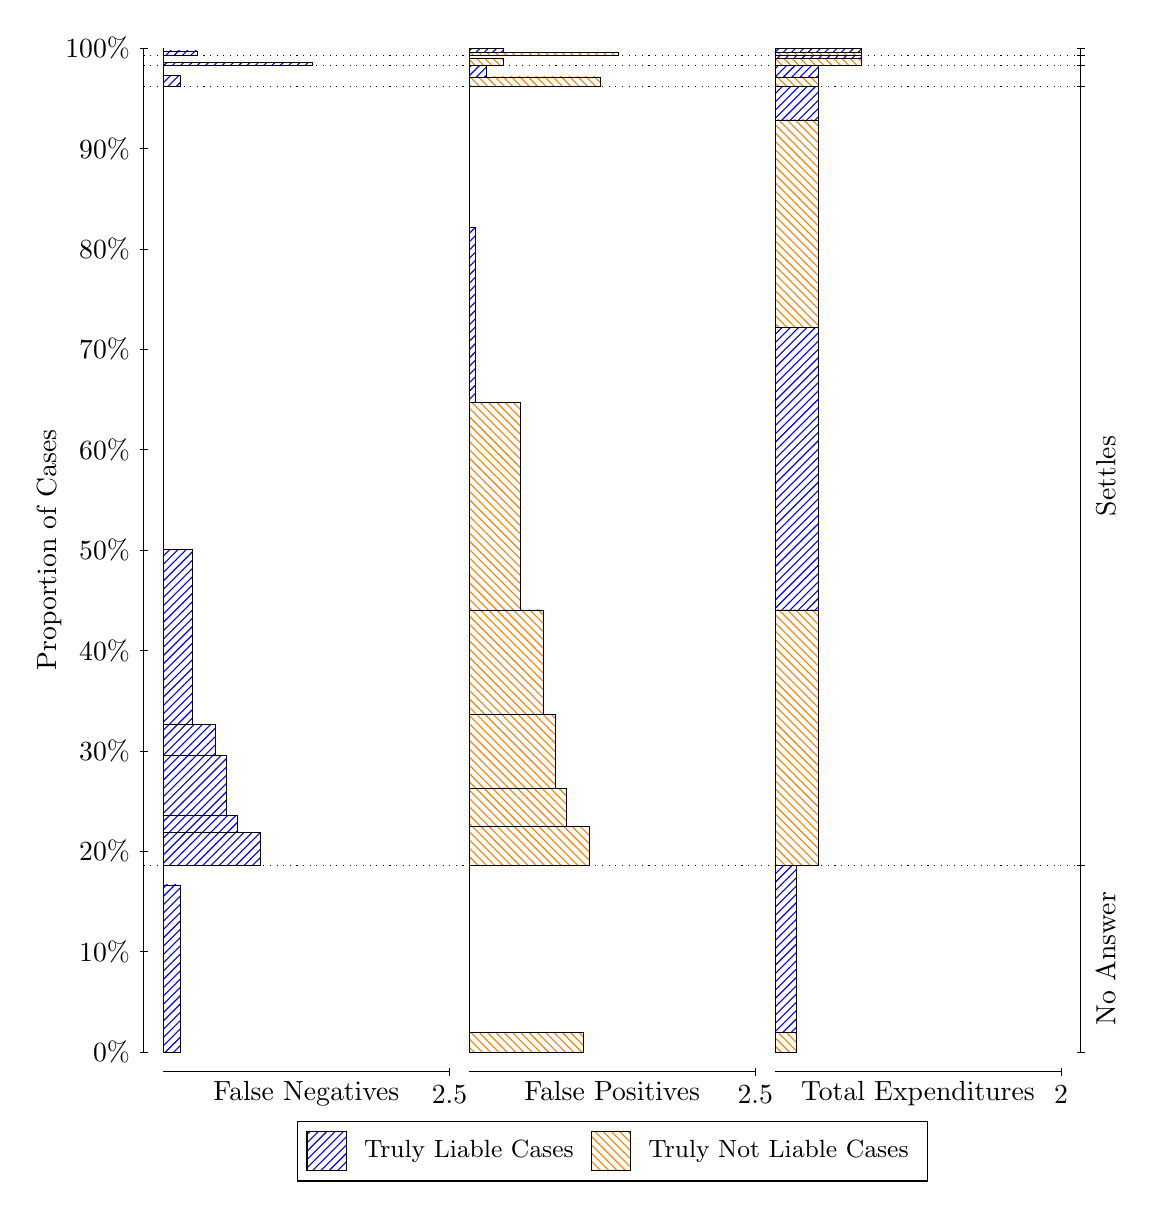
\begin{tikzpicture}
\draw[black, very thin] (1.5,1.75) -- (1.5,14.5);
\node[rotate=90, text=black, anchor=center] at (0.3, 8.125) {Proportion of Cases};
\draw[black, very thin] (1.45,1.75) -- (1.55,1.75);
\node[text=black, anchor=east] at (1.45, 1.75) {0\%};
\draw[black, very thin] (1.45,3.025) -- (1.55,3.025);
\node[text=black, anchor=east] at (1.45, 3.025) {10\%};
\draw[black, very thin] (1.45,4.3) -- (1.55,4.3);
\node[text=black, anchor=east] at (1.45, 4.3) {20\%};
\draw[black, very thin] (1.45,5.575) -- (1.55,5.575);
\node[text=black, anchor=east] at (1.45, 5.575) {30\%};
\draw[black, very thin] (1.45,6.85) -- (1.55,6.85);
\node[text=black, anchor=east] at (1.45, 6.85) {40\%};
\draw[black, very thin] (1.45,8.125) -- (1.55,8.125);
\node[text=black, anchor=east] at (1.45, 8.125) {50\%};
\draw[black, very thin] (1.45,9.4) -- (1.55,9.4);
\node[text=black, anchor=east] at (1.45, 9.4) {60\%};
\draw[black, very thin] (1.45,10.675) -- (1.55,10.675);
\node[text=black, anchor=east] at (1.45, 10.675) {70\%};
\draw[black, very thin] (1.45,11.95) -- (1.55,11.95);
\node[text=black, anchor=east] at (1.45, 11.95) {80\%};
\draw[black, very thin] (1.45,13.225) -- (1.55,13.225);
\node[text=black, anchor=east] at (1.45, 13.225) {90\%};
\draw[black, very thin] (1.45,14.5) -- (1.55,14.5);
\node[text=black, anchor=east] at (1.45, 14.5) {100\%};

\draw[black, very thin] (13.4,1.75) -- (13.4,14.5);
\draw[black, very thin] (13.35,1.75) -- (13.45,1.75);
\node[anchor=west] at (13.35, 1.75) {};
\draw[black, very thin] (13.35,4.1222) -- (13.45,4.1222);
\node[anchor=west] at (13.35, 4.1222) {};
\draw[black, very thin] (13.35,14.009) -- (13.45,14.009);
\node[anchor=west] at (13.35, 14.009) {};
\draw[black, very thin] (13.35,14.282) -- (13.45,14.282);
\node[anchor=west] at (13.35, 14.282) {};
\draw[black, very thin] (13.35,14.406) -- (13.45,14.406);
\node[anchor=west] at (13.35, 14.406) {};
\draw[black, very thin] (13.35,14.5) -- (13.45,14.5);
\node[anchor=west] at (13.35, 14.5) {};

\draw[black, very thin, pattern color=blue, pattern=north east lines] (1.75,1.75) rectangle (1.968,3.8726);
\draw[black, very thin, pattern color=orange, pattern=north west lines] (1.75,3.8726) rectangle (1.75,4.1222);
\draw[black, very thin, pattern color=blue, pattern=north east lines] (1.75,4.1222) rectangle (2.9853,4.5423);
\draw[black, very thin, pattern color=blue, pattern=north east lines] (1.75,4.5423) rectangle (2.6947,4.7541);
\draw[black, very thin, pattern color=blue, pattern=north east lines] (1.75,4.7541) rectangle (2.5493,5.5207);
\draw[black, very thin, pattern color=blue, pattern=north east lines] (1.75,5.5207) rectangle (2.404,5.9092);
\draw[black, very thin, pattern color=blue, pattern=north east lines] (1.75,5.9092) rectangle (2.1133,8.1319);
\draw[black, very thin, pattern color=orange, pattern=north west lines] (1.75,8.1319) rectangle (1.75,14.009);
\draw[black, very thin, pattern color=blue, pattern=north east lines] (1.75,14.009) rectangle (1.968,14.157);
\draw[black, very thin, pattern color=orange, pattern=north west lines] (1.75,14.157) rectangle (1.75,14.282);
\draw[black, very thin, pattern color=blue, pattern=north east lines] (1.75,14.282) rectangle (3.6393,14.319);
\draw[black, very thin, pattern color=orange, pattern=north west lines] (1.75,14.319) rectangle (1.75,14.406);
\draw[black, very thin, pattern color=blue, pattern=north east lines] (1.75,14.406) rectangle (2.186,14.463);
\draw[black, very thin, pattern color=orange, pattern=north west lines] (1.75,14.463) rectangle (1.75,14.5);
\draw[black, very thin, pattern color=orange, pattern=north west lines] (5.6333,1.75) rectangle (7.0867,1.9996);
\draw[black, very thin, pattern color=blue, pattern=north east lines] (5.6333,1.9996) rectangle (5.6333,4.1222);
\draw[black, very thin, pattern color=orange, pattern=north west lines] (5.6333,4.1222) rectangle (7.1593,4.6148);
\draw[black, very thin, pattern color=orange, pattern=north west lines] (5.6333,4.6148) rectangle (6.8687,5.0929);
\draw[black, very thin, pattern color=orange, pattern=north west lines] (5.6333,5.0929) rectangle (6.7233,6.0418);
\draw[black, very thin, pattern color=orange, pattern=north west lines] (5.6333,6.0418) rectangle (6.578,7.364);
\draw[black, very thin, pattern color=orange, pattern=north west lines] (5.6333,7.364) rectangle (6.2873,9.9988);
\draw[black, very thin, pattern color=blue, pattern=north east lines] (5.6333,9.9988) rectangle (5.706,12.221);
\draw[black, very thin, pattern color=blue, pattern=north east lines] (5.6333,12.221) rectangle (5.6333,14.009);
\draw[black, very thin, pattern color=orange, pattern=north west lines] (5.6333,14.009) rectangle (7.3047,14.133);
\draw[black, very thin, pattern color=blue, pattern=north east lines] (5.6333,14.133) rectangle (5.8513,14.282);
\draw[black, very thin, pattern color=orange, pattern=north west lines] (5.6333,14.282) rectangle (6.0693,14.369);
\draw[black, very thin, pattern color=blue, pattern=north east lines] (5.6333,14.369) rectangle (5.6333,14.406);
\draw[black, very thin, pattern color=orange, pattern=north west lines] (5.6333,14.406) rectangle (7.5227,14.443);
\draw[black, very thin, pattern color=blue, pattern=north east lines] (5.6333,14.443) rectangle (6.0693,14.5);
\draw[black, very thin, pattern color=orange, pattern=north west lines] (9.5167,1.75) rectangle (9.7892,1.9996);
\draw[black, very thin, pattern color=blue, pattern=north east lines] (9.5167,1.9996) rectangle (9.7892,4.1222);
\draw[black, very thin, pattern color=orange, pattern=north west lines] (9.5167,4.1222) rectangle (10.062,7.364);
\draw[black, very thin, pattern color=blue, pattern=north east lines] (9.5167,7.364) rectangle (10.062,10.954);
\draw[black, very thin, pattern color=orange, pattern=north west lines] (9.5167,10.954) rectangle (10.062,13.588);
\draw[black, very thin, pattern color=blue, pattern=north east lines] (9.5167,13.588) rectangle (10.062,14.009);
\draw[black, very thin, pattern color=orange, pattern=north west lines] (9.5167,14.009) rectangle (10.062,14.133);
\draw[black, very thin, pattern color=blue, pattern=north east lines] (9.5167,14.133) rectangle (10.062,14.282);
\draw[black, very thin, pattern color=orange, pattern=north west lines] (9.5167,14.282) rectangle (10.607,14.369);
\draw[black, very thin, pattern color=blue, pattern=north east lines] (9.5167,14.369) rectangle (10.607,14.406);
\draw[black, very thin, pattern color=orange, pattern=north west lines] (9.5167,14.406) rectangle (10.607,14.443);
\draw[black, very thin, pattern color=blue, pattern=north east lines] (9.5167,14.443) rectangle (10.607,14.5);
\draw[black, dotted] (1.5,4.1222) -- (13.4,4.1222);
\draw[black, dotted] (1.5,14.009) -- (13.4,14.009);
\draw[black, dotted] (1.5,14.282) -- (13.4,14.282);
\draw[black, dotted] (1.5,14.406) -- (13.4,14.406);
\draw[black, very thin] (1.75,1.5) -- (5.3833,1.5);
\node[text=black, anchor=north] at (3.5667, 1.5) {False Negatives};
\draw[black, very thin] (5.3833,1.45) -- (5.3833,1.55);
\node[text=black, anchor=north] at (5.3833, 1.45) {2.5};

\draw[black, very thin] (5.6333,1.5) -- (9.2667,1.5);
\node[text=black, anchor=north] at (7.45, 1.5) {False Positives};
\draw[black, very thin] (9.2667,1.45) -- (9.2667,1.55);
\node[text=black, anchor=north] at (9.2667, 1.45) {2.5};

\draw[black, very thin] (9.5167,1.5) -- (13.15,1.5);
\node[text=black, anchor=north] at (11.333, 1.5) {Total Expenditures};
\draw[black, very thin] (13.15,1.45) -- (13.15,1.55);
\node[text=black, anchor=north] at (13.15, 1.45) {2};

\node[text=black, centered, rotate=90] at (13.72, 2.9361) {No Answer};
\node[text=black, centered, rotate=90] at (13.72, 9.0654) {Settles};




\draw (7.449999999999999,1.5) node[draw=none] (baseCoordinate) {};
\begin{scope}[align=center]
        \matrix[scale=0.5, draw=black, below=0.5cm of baseCoordinate, nodes={draw}, column sep=0.1cm]{
            \node[rectangle, draw, minimum width=0.5cm, minimum height=0.5cm, pattern color=blue, pattern=north east lines] {}; &
            \node[draw=none, font=\small, text=black] (B) {Truly Liable Cases}; &
            \node[rectangle, draw, minimum width=0.5cm, minimum height=0.5cm, pattern color=orange, pattern=north west lines] {}; &
            \node[draw=none, font=\small, text=black] (B) {Truly Not Liable Cases}; \\
            };
\end{scope}

\end{tikzpicture}
\end{document}